% Author : Kevin Coulomb 
% Date   : 09/02/2011
% Email  : kevin.coulomb@sysfera.com
% Version: 1.0
\documentclass{article}

\usepackage[english]{babel}
\usepackage{graphicx}

\begin{document}
The aim of this document is to present the registry of mapper solution.

\section*{Presentation}
The registry of mapper represents the a register used to keep track of the 
various modules that are used and the commands that are within them. The 
register is representated by a singleton class that contains a map of the 
mappers and their name. There is one mapper per module (e.g. UMS has its own
mapper, FMS has its own mapper, etc...). The mapper class represents an 
interface that contains a map of key (string) and commands (string) and some 
public functions to get the correspondances between the key and the command. 
The aim of a mapper is to link the commands with their key to make possible a 
generic storage of the commands typed by the user within the VISHNU system. 

Each module will have its mapper and will register in the mapper registry. Each 
time a user type a command of the module, the command is registered following 
the mapper code in the database. When the user wants the list of its commands, 
he gets their code from the database and can get the corresponding function call.
This is made to easily get the right function call, without having to parse to go 
from one format to another.

\section*{Classes}

\begin{figure}[h]
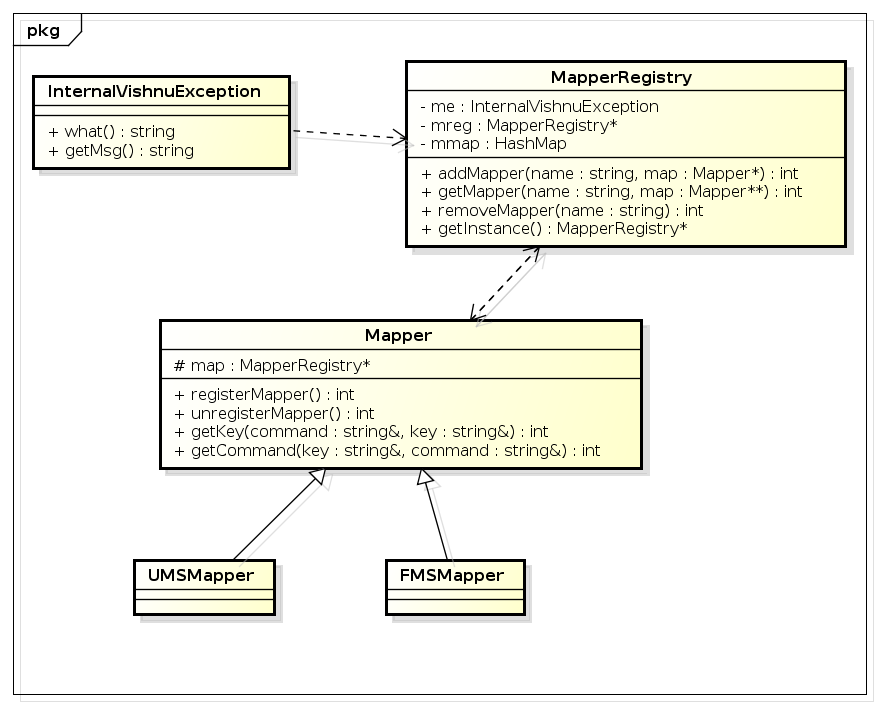
\includegraphics[scale=0.8, angle=90]{image/mapperRegistry.png}
\caption{Class diagram for the registry module}
\end{figure}

The class diagram schema represents all the public methods et attributes of the 
module.
The InternalVishnuException class is the kind of exception that can be returned
by the module, for more information about the exception mecanism, please refer 
to the document presenting the exceptions.
The MapperRegistry is a singleton, so it has a static pointer to the only 
accessible instance, an exception object, and a map of the available mappers.
The map has the module names as key and a pointer to the corresponding mapper as 
an argument. If one tries to add an already existing mapper, he is not added and 
success is returned.

The Mapper class is an interface that defines what a mapper can do. It has a 
pointer to the mapper registry (althougt not necessary, i prefer to store it 
rather than always calling the get instance method).
The class has a protected map, that will be inherited and used by the 
realizations of the class.
The map is composed by two strings, a key number that will be used to manipulate 
abstract data, and the real value of the key (=the command).

For instance, mapper will have two subclasses, one called UMSMapper and one 
called FMSMapper.
\end{document}
